\documentclass{baer}
%%%%%%%%%%%%%%%%%%%%%%%%%%%%
% NEL CASO IN CUI LA TESI E' REDATTA IN INGLESE
% Commentare la riga precedente e scommentare la seguente
%\documentclass{baer_en}
%%%%%%%%%%%%%%%%%%%%%%%%%%%%


%%%%%%%%%%%%%%%%%%%%%%%%%%%%
% una delle due seguenti righe deve essere attiva per includere i caratteri accentati nel file
%%%%%%%%%%%%%%%%%%%%%%%%%%%%
%\usepackage[latin1]{inputenc}
\usepackage[utf8]{inputenc}
%%%%%%%%%%%%%%%%%%%%%%%%%%%


%%%%%%%%%%%%%%%%%%%%%%%%%%%
% qui si possono inserire ulteriori packages 
% si ricorda che i packages:
% graphicx, color, amssymb, amsmath, latexsym,
% amsthm, babel (italian)
% sono già inclusi in baer.cls
%%%%%%%%%%%%%%%%%%%%%%%%%%%

%%%%%%%%%%%%%%%%%%%%%%%%%%%
% Dati del candidato e della tesi
%%%%%%%%%%%%%%%%%%%%%%%%%%%
\candidato{Nome Cognome}
\matricola{numero di matricola}
\relatore{Carlo Massimo Casciola}
\correlatore{Andrea Gallegati}
\ssd{ING-IND/06 FLUIDODINAMICA}
\title{Titolo dell'elaborato finale}
%%%%%%%%%%%%%%%%%%%%%%%%%%%

 
\abstract{
In questa sezione il candidato illustra un riassunto del lavoro svolto
mettendone in evidenza le parti degne di maggior attenzione da parte del relatore
e della commissione di laurea. La stesura e l'abilità nel redigere tale abstract
costituiscono parte integrante della valutazione complessiva. Il candidato può
sovrascrivere questo template avendo cura di non modificarne la formattazione. Il
font è {\bf Arial 10} per il testo.
}

\begin{document}
\maketitle

\section{Introduzione}



Il titolo dei paragrafi è in \textbf{bold} ed il font è sempre \textbf{Arial 10}.
L’intero documento deve essere redatto limitandone la
lunghezza ad un \textbf{massimo di 7 pagine} del presente form
– template (da riempire), incluse le figure, \textbf{senza alcuna
eccezione, e deve essere rilegato a spirale con trasparente anteriore e cartoncino posteriore}.

\section{Tipologia del lavoro}

L’elaborato finale è svolto individualmente dall’allievo ed
in completa autonomia, sotto la supervisione di un
relatore che propone e verifica i contenuti.\\
Per sostenere l’esame finale l’allievo consegna
ufficialmente il documento al Presidente della
commissione di Laurea.\\
Il relatore può far riferimento a diverse tipologie di lavoro
(puramente indicative), che si riportano a seguire, purché
si mantenga la fondamentale nozione del valore dei 5
CFU in palio.

\subsection{Paper review}
Consiste nella sintesi di un articolo scelto di comune
accordo tra l’allievo ed il relatore, da una rivista o dagli
atti di un congresso, preferibilmente dalla letteratura
internazionale; l’elaborato deve contenere, in sintesi, tutti
gli aspetti più importanti esposti nell’articolo: argomento,
novità proposta, metodologia, risultati e si dovrà
concludere con una nota critica sviluppata
autonomamente dall’allievo.

\subsection{Code report}
Consiste nella stesura di un programma di calcolo
autonomamente sviluppato dall’allievo che verrà
presentato al relatore; l’elaborato da consegnare consiste
in un codice di calcolo con linee di commento che
illustrino chiaramente i parametri input ed output, il
metodo e l’utilità.

\subsection{Model development}
Come per il Code report, ma sviluppato in un ambiente di
programmazione commerciale (SolidWorks, AutoCAD,
Ansys, MSC.Nastran, CFD++, Star, Matlab/Simulink,
Scilab o altro).

\subsection{Test report}
Consiste in un piccolo lavoro sperimentale svolto in un
laboratorio della Sapienza o esterno, cui seguirà un
report con la descrizione dell’attività sperimentale, catena
di misura, accuratezza, risultati, affidabilità.

\subsection{Team partnership}
Con riferimento alla competizione AIAA DBF o altre
equivalenti (tenendo sempre conto dei 5 CFU) e con
possibilità di diffondere notizie riguardanti il team e i
progressi del progetto (con la riservatezza richiesta dalla
competizione).

\subsection{Approfondimento didattico}
Si intende l’approfondimento di un argomento trattato in
un corso curriculare, basato sulla consultazione di
ulteriori testi oltre quelli consigliati, sia di tipo cartaceo
che elettronico. Può prevedere la spiegazione di un certo
argomento con diverse metodologie, oppure la
preparazione di esercizi di tipo didattico utili alla
comprensione e all’applicazione dei concetti teorici,
oppure la descrizione di una specifica applicazione.

\section{Esempio di paragrafo}

I simboli delle grandezze devono essere scritti in carattere \textit{corsivo}, tanto nelle formule che nel testo; le unità di misura ed i simboli delle specie chimiche devono invece essere riportati in carattere normale (ad esempio km, H$_2$O, K, $^{\rm o}$C, gli ultimi due relativi a gradi Kelvin e Celsius, rispettivamente), come pure gli operatori matematici (ad esempio log, exp, sin, cos, etc.). Tutte le formule devono essere numerate progressivamente (a destra), ad esempio

\begin{equation}
F = m \: a
\label{e:forza}
\end{equation}

\begin{equation}
\cfrac{m_f}{m_0}=\exp\left(-\cfrac{\Delta v}{u_{eq}}\right)
\label{e:massratio}
\end{equation}

\noindent e sono richiamate nel testo come (ad esempio) "La forza $F$ è data dall'eq.~(\ref{e:forza}), ...".

\smallskip 


\noindent Tutte le figure devono essere numerate e devono includere una didascalia \textbf{esplicativa} (che cioè deve chiarirne il significato), ed eventualmente, se sono riprese da un testo, indicare il riferimento bibliografico a questo relativo, ad esempio

\begin{figure}[h]
\centerline{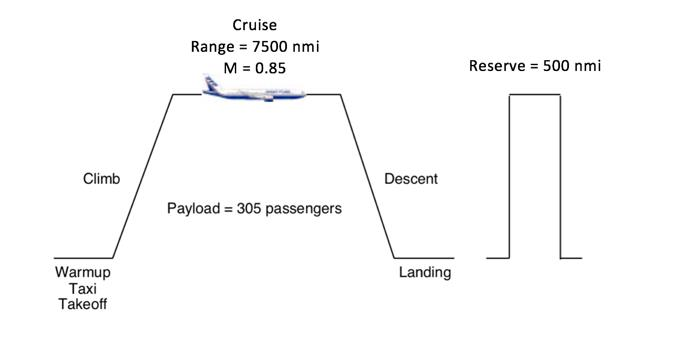
\includegraphics[width=0.9\columnwidth]{B777.jpg}}
\caption{Tipico profilo di missione di un Boeing 777-200ER, da~\protect{\cite{dirks04}}.}
\label{f:B777}
\end{figure} 

La figura sarà richiamata nel testo come, ad esempio, "dalla fig.~\ref{f:B777} si osserva..."  (e \textit{non}, ad esempio, "dalla figura \textit{sotto} si osserva...").

\smallskip 

\noindent Tutte le figure e le tabelle \textit{devono} essere citate nel testo.

\smallskip 

\noindent Tutte le tabelle devono essere numerate e devono includere una didascalia esplicativa, vedi ad esempio la tab.~\ref{t:sistprop}, e devono essere richiamate nel testo come (ad esempio) "come si deduce dalla tab.~\ref{t:sistprop}...".

\begin{table}
\begin{center}
\begin{tabular}{|c|c|c|c|} \hline
 \textit{Aereo}          & \begin{tabular}{c} \textit{n.} \\ \textit{motori}\end{tabular} & \begin{tabular}{c} \textit{spinta}\\  \textit{individuale} \\(kN)\end{tabular}  & \begin{tabular}{c} \textit{anno di} \\ \textit{introduzione} \\ \textit{in servizio}\end{tabular} \\  \hline
Boeing 707   &  4           &                  80              &  1959    \\ \hline
Boeing 727   &  3           &                  62              &  1964    \\ \hline
Boeing 737   &  2           &                  62              &  1968    \\ \hline
Boeing 747   &  4           &                 206              &  1970    \\ \hline
Boeing 757   &  2           &                 179              &  1983    \\ \hline
Boeing 767   &  2           &                 214              &  1982    \\ \hline
Boeing 777   &  2           &                 343              &  1995    \\ \hline
Boeing 787   &  2           &                 280              &  2011    \\ \hline
\end{tabular}
\caption{Caratteristiche del sistema propulsivo di alcuni aerei da trasporto commericiali.}\label{t:sistprop}
\end{center}
\end{table}


 

\section{Conclusioni}
Sarà opportuno concludere l’elaborato con un paragrafo dal quale
si possano apprezzare in sintesi il lavoro svolto ed i
risultati raggiunti.


%\bibliography{my_library}
%\bibliographystyle{baer}

\begin{thebibliography}{99}
% Commentare mediante un % i commenti esplicativi
\bibitem[Per il materiale utilizzato o consultato, tratto da internet o]{}
da un paper, ivi compresi risultati, foto, immagini e
disegni non prodotti dal Candidato, è  \textbf{necessario}
elencare appropriata bibliografia di riferimento, o i siti
web consultati. Tutti i riferimenti riportati nella bibliografia
devono essere citati nel testo della tesi. Il riferimento va
fatto in ordine di apparizione e l’elenco va compilato 
seguendo  \textit{strettamente} il seguente schema:

Per i libri:

\bibitem{sutton01} Sutton, G.P. e Biblarz, O., \textit{Rocket Propulsion Elements}, 7th ed., Wiley, New York, 2001.

[cognome del primo autore, iniziali del suo nome, cognome del secondo autore (eventuale), iniziali, etc., fino all'ultimo autore, \textit{Titolo del libro} (\textit{in corsivo}), eventuale n. dell'edizione, casa editrice, sede (città) della  casa editrice, anno di pubblicazione. Eventualmente si possono specificare le pagine, ad esempio ... New York, 2001, pp. 211-221]. 

Per gli articoli su rivista:

\bibitem{lolis14} Lolis, P., Giannakakis, P. , Sethi, V., Jackson, A.J.B. e Pilidis, P., Evaluation of aero gas turbine preliminary weight estimation methods, \textit{The Aeronautical J.}, vol. 118, pp. 625-641, 2014.

[cognome del primo autore, iniziali, etc., titolo dell'articolo (in carattere normale), nome della rivista (\textit{in corsivo}) abbreviato (esistono abbrevazioni standard per ciascuna rivista), numero del volume, (talvolta viene indicato anche il numero del fascicolo che compone il dato volume, non necessario), numero delle pagine (sempre), anno di pubblicazione].

Per i rapporti:

\bibitem{marte70} Marte, J.E. e Kurtz, D.W., A review of aerodynamic noise from propellers, rotors, and lift fans, Jet Propulsion Laboratory Tech. Rept. 32-1462, 1970.

[autori, iniziali, etc., titolo del rapporto, ente, numero/codice del rapporto, anno].

Per gli articoli presentati in conferenze (eccetto AIAA, IAC, SAE, vedi oltre):

\bibitem{dirks04} Dirks, G.A., Noise - a driver for change, 8th ASC-CEAS workshop, Budapest, 2004.

Per gli articoli presentati in conferenze AIAA (American Institute of Aeronautics and Astronautics):

\bibitem{gern05} Gern, F.H., Ko, A., Grossman, B., Haftka, R.Y., Kapania, R.K. e Mason, W.H., Transport weight reduction through MDO: the strut-braced wing transonic transport, AIAA-2005-4667, 2005.

(autori, titolo, numero del paper AIAA nel formato AIAA-anno-numero progressivo, anno; gli articoli degli anni precedenti il 2000 seguono il formato AIAA-98-0438, 1998).

Per gli articoli presentati in congressi IAC (International Astronautical Congress):

\bibitem{summerer11} Summerer, L. e Jacques, L., Prospects for space solar power in Europe, IAC-11-C3.1.3, 2011.

(autori, titolo, numero del paper IAC nel formato IAC-numero progressivo, anno).

Per gli articoli presentati in conferenze SAE (Society of Automotive Engineers):

\bibitem{kirby99} Kirby, M.R. e Mavris, D.N., Forecasting technology uncertainty in preliminary aircraft design, SAE 1999-01-5631, 1999.

(autori, titolo, numero del paper SAE nel formato SAE numero progressivo, anno).

Per un capitolo di un \textit{edited book} (libro in cui ciascun capitolo è scritto da autori diversi, coordinati da uno - o più - \textit{editors}):

\bibitem{turchi95} Turchi, P.J., Electric rocket propulsion systems, cap. 10 in \textit{Space Propulsion Analysis and Design} (Humble, R.W., Henry, G.N. e Larson, W.J., Ed.), McGraw-Hill, New York, 1995.

(notare il titolo del libro in corsivo, e la specifica "Ed." che designa Humble Henry e Larson come \textit{editors}).

Per i siti web:

\bibitem{vulcain} Website www.space-propulsion.com/launcher-propulsion/rocket-engines/vulcain-rocket-engine.html\#moved, consultato il gg.mm.aaaa.

Per i lavori non pubblicati:

\bibitem{dorrington15} Dorrington, G.E., Speculation on fuelling commercial air transportation in 2050, non pubblicato, 2015.

Per comunicazioni personali:

\bibitem{russo17} Russo, A., comunicazione personale, 2017.

Per dispense di un corso:

\bibitem{spagnolo17} Spagnolo, B., Dispense del corso di Motori termici, Università di Perugia, 2017.

Per presentazioni:

\bibitem{devinder15} Devinder, K.Y., Gas turbine theory - thrust augmentation and noise suppression, presentazione, 2015.

\end{thebibliography}




\appendix
\section{Appendice}

Le eventuali appendici vanno poste dopo la bibliografia e, se più di una, contraddistinte da lettere in ordine progressivo, A, B, etc.

\bigskip


L’elaborato o il codice di calcolo, se ritenuti dal relatore
meritevoli di particolare attenzione, potranno essere
pubblicati su una sezione dedicata del sito del CAD
Aerospaziale (Wikiaerospace) per consultazione da
parte di studenti e personale di aziende interessate.

\section{Redazione della tesi in LaTeX}
Per la redazione della tesi in LaTeX è disponibile un file di esempio:
\begin{verbatim} Template_Elaborato_Finale_BAER_2019.tex \end{verbatim} 
insieme ai files necessari rispettare lo stile previsto per il documento.
L'insieme dei files è il seguente:
\begin{itemize}
 \item \verb=Template_Elaborato_Finale_BAER_2019.tex= (File di esempio)
 \item \verb=baer.cls= (Stile del documento)
 \item \verb=baer_en.cls= (Stile del documento se redatto in inglese)
 %\item \verb=baer.bst= (Stile della bibliografia)
 %\item \verb=my_library.bib= (File esempio per i riferimenti bibliografici e sitografici)
 \item \verb=sap.jpg= (Immagine necessaria per l'intestazione della prima pagina)
 \item \verb=ici.jpg= (Immagine necessaria per l'intestazione delle pagine successive)
 \item \verb=B777.jpg= (Esempio di figura)
 \item \verb=Template_Elaborato_Finale_BAER_2019.pdf= (File pdf di questo documento preparato con LaTeX)
\end{itemize}
I files sono preparati per la compilazione con pdflatex. % e bibtex. 
Ad esempio, da linea di comando,  
per permettere la corretta distribuzione di tutti i riferimenti incrociati e della bibliografia è necessario 
utilizzare la sequenza (ripetendo quindi due volte):\\
\begin{verbatim} 
pdflatex Template_Elaborato_Finale_BAER_2019 
pdflatex Template_Elaborato_Finale_BAER_2019 
\end{verbatim}
%bibtex template_tesi 
%pdflatex template_tesi 

\section{English version}
If thesis is written in English, the candidate should change the 
document class from \verb=baer.cls= to \verb=baer_en.cls=. 
Note that the headings of the first page (``Elaborato finale \ldots'', ``Candidato'', 
\ldots) will remain unchanged.


\end{document}
